Como parte simplificada de la estructura de una comunidad de nodos en una red social, cada uno representa a un individuo y la red tiene una segmentación multitudinaria~\cite{ma2014exploring}. Algunas personas son centrales en la comunidad, algunas están al margen, establecen menos relaciones con otros y, por lo tanto, tienen una influencia menor. En esta sección, presentamos un nuevo enfoque de descubrimiento comunitario basado en el algoritmo PageRank para encontrar a estos delincuentes "importantes" ó con "mayor influencia" en nuestro grafo, con el fin de analizar supuestas bandas delictivas.

\subsubsection{Definición formal de Grafo}
Un grafo es un par $G = (N, A, g)$ donde $N$ es un conjunto finito no vacío de elementos denominados \textit{nodos} (vértices), $A$ es un conjunto de arcos y $g$ es una función que asocia a cada arco $a$ perteneciente a $A$ con un par no ordenado $(x, y)$, siendo $x$ e $y$ nodos pertenecientes a $N$. Se dice que $a$ es un arco con vértices extremos $x$ e $y$~\cite{dubinsky1984mathematical}.

\subsubsection{PageRank}
(PR) es un método que fue implementado a través de un algoritmo
originalmente utilizado por Google que asigna a cada página web de un conjunto dado, un puntaje que refleja su importancia dentro del conjunto. A este puntaje se lo denomina \textit{valor de PageRank}. Ante una consulta, el buscador utiliza estos puntajes para determinar el nivel de relevancia de las páginas, y retorna en primer lugar aquellas con un puntaje más alto. Para calcular los puntajes, PageRank utiliza la estructura de enlaces de la web~\cite{brin1998anatomy}. Una página web tiene un valor de PageRank alto si es apuntada por muchas otras páginas, o bien si es apuntada por páginas con puntajes altos~\cite{page1999pagerank}. PageRank tiene una base intuitiva en el concepto de \textit{random walks} sobre grafos~\cite{gobel1974random}: supongamos que un navegante aleatorio empieza a navegar la web desde una página cualquiera. El navegante puede hacer clic en forma aleatoria sobre alguno de los enlaces presentes en la página en la que se encuentra actualmente con una probabilidad $d$ a la que se denomina \textit{damping factor}, o bien con probabilidad $1-d$ accede aleatoriamente a cualquier otra página web. Este proceso se repite indefinidamente. Luego, el valor de PageRank de una página $P$ puede ser interpretado como la probabilidad de que el navegante aleatorio se encuentre en $P$ al finalizar el proceso. PageRank es definido formalmente de la siguiente manera ~\cite{franceschet2011pagerank}. Sean $q_i$ el número de enlaces salientes que posee la página $i$ , $n$ el número total de páginas web, $d$ el \textit{damping factor} que por lo general adquiere el valor 0.85, $\pi$ un vector columna denominado \textit{vector PageRank}, y $H = (h_{ij})$ una matriz cuadrada de tamaño $n$ tal que $h_{ij} = 1/q_i$ si existe un enlace desde la página $i$ a la página $j$ , y $h_{ij} = 0$ en caso contrario. El valor $h_{ij}$ corresponde a la probabilidad de acceder a la página $j$ desde la página $i$ en un paso, a partir de hacer clic en alguno de los enlaces que aparecen en esta última. El valor de PageRank correspondiente a la página $j$ es $\pi_j$, y se define recursivamente como se muestra en la ecuación \ref{eqn:ecuacionPageRank}~\cite{lin2010data}.

\begin{equation} 
	\label{eqn:ecuacionPageRank} 
	\pi_j = \frac{1-d}{n} + d \sum_{i=1}^{n} \pi_i h_{ij} 
\end{equation}

\subsubsection{Aplicación de PageRank para bandas delictivas}
Nuestro dataset descrito anteriormente se obtiene a partir de consultas SQL a la Base de Datos de Coirón. Para hacer uso del algoritmo de PageRank se decidió incorporarlo dentro de esas consultas SQL de modo de obtener un resultado que pueda ser utilizado para la visualización. Dentro de la consulta original se generaba una tabla para los nodos y otra tabla para las relaciones, de esta manera el software realizado para la visualización obtiene dichos datasets y renderiza el grafo.
Para incorporar el cálculo de PageRank, inicialmente se adecuaron ambas tablas para la utilización de la fórmula, y se necesitó de ciertas tablas temporales para el cálculo. Por un lado se computó el grado de salida de cada nodo \textit{(Out Degree)}, es decir el número de enlaces que lo conectan con otros nodos.

\begin{verbatim}
INSERT INTO #OutDegree
	SELECT #Node.id, COUNT(#Edge.src)
	FROM #Node 
		LEFT OUTER JOIN #Edge ON #Node.id = #Edge.src
	GROUP BY #Node.id		
\end{verbatim}

Luego se declara el \textit{damping factor}, en nuestro caso $0.85$, el conteo total de nodos, y se calcula el \textit{PageRank inicial} de cada nodo, para después comenzar la iteración buscando cumplir con la sumatoria de la fórmula.

\begin{verbatim}
DECLARE @dampingFactor float = 0.85
DECLARE @Node_Num int
SELECT @Node_Num = COUNT(*) FROM #Node
INSERT INTO #PageRank
	SELECT #Node.id, rank = ((1 - @dampingFactor) / @Node_Num)
	FROM #Node 
		INNER JOIN #OutDegree ON #Node.id = #OutDegree.id
DECLARE @Iteration int = 0
WHILE @Iteration < 50
BEGIN
	--Iteration Style
	SET @Iteration = @Iteration + 1
	INSERT INTO #TmpRank
		SELECT #Edge.dst, rank = ((1 - @dampingFactor) / @Node_Num) 
		+ (@dampingFactor * SUM(#PageRank.rank / #OutDegree.degree))
		FROM #PageRank 
			INNER JOIN #Edge ON #PageRank.id = #Edge.src
			INNER JOIN #OutDegree ON #PageRank.id = #OutDegree.id
		GROUP BY #Edge.dst
END
\end{verbatim}

Una vez finalizado el desarrollo de la fórmula, se procedió a realizar pruebas que corroboren el buen funcionamiento del código. Se realizaron ejemplos para pocos nodos con pocas relaciones, de manera tal que sea sencilla la verificación. Se muestran a continuación el Cuadro \ref{tab:TablaPageRank6Nodos} con los resultados de PageRank para 6 nodos, y la Figura \ref{fig:6nodos-pageRank-sinColor} que refleja la visualización de la misma ejecución. En cada nodo se muestra su posición de PageRank, y entre paréntesis el identificador de cada nodo. Como se puede observar el nodo central por el PageRank calculado es el referido al ID \textit{145053}, cuyas relaciones con 3 nodos pesan sobre las relaciones que poseen el resto de los nodos visualizados en el grafo.

\begin{table}
\centering
\label{tab:TablaPageRank6Nodos}
\begin{tabular}{|l|r|}
	\hline
	\textbf{IdNodo} &  \textbf{PageRank} \\
	\hline
	145053 &  0,286845042094944 \\
	\hline
	145262 &  0,199512347112651 \\
	\hline
	116587 &  0,1910604814502 \\
	\hline
	132310 &  0,109790233522352 \\
	\hline
	123109 &  0,106270247927848 \\
	\hline
	129137 &  0,106270247927848 \\
	\hline
\end{tabular}
\vspace{10pt}
\caption{Valores de PageRank por nodo luego de la ejecución del algoritmo}
\end{table}

\begin{figure}
	\centering
	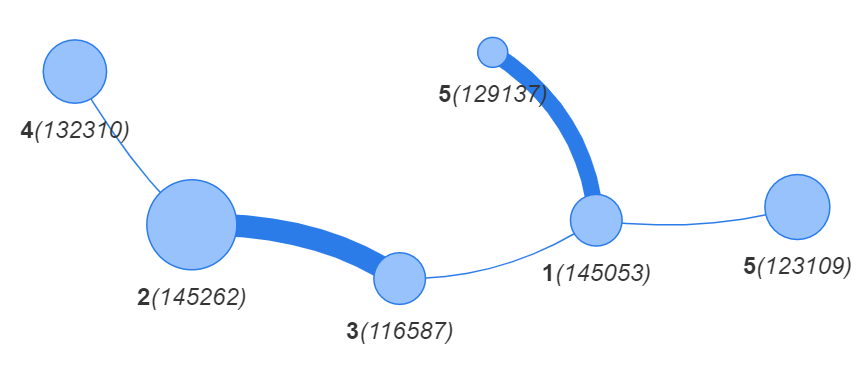
\includegraphics[width=0.75\linewidth]{6nodos-pageRank-sinColor.png}
	\caption{Resultado de ejecución de PageRank para 6 nodos.} 
	\label{fig:6nodos-pageRank-sinColor}
\end{figure}



